% !TeX root = probability.tex

%%%%%%%%%%%%%%%%%%%%%%%%%%%%%%%%%%%%%%%%%%%%%%%%%%%%%%%%%%%%%%

\section{קיץ תשע"ט מועד ב}

\begin{center}
\selectlanguage{english}
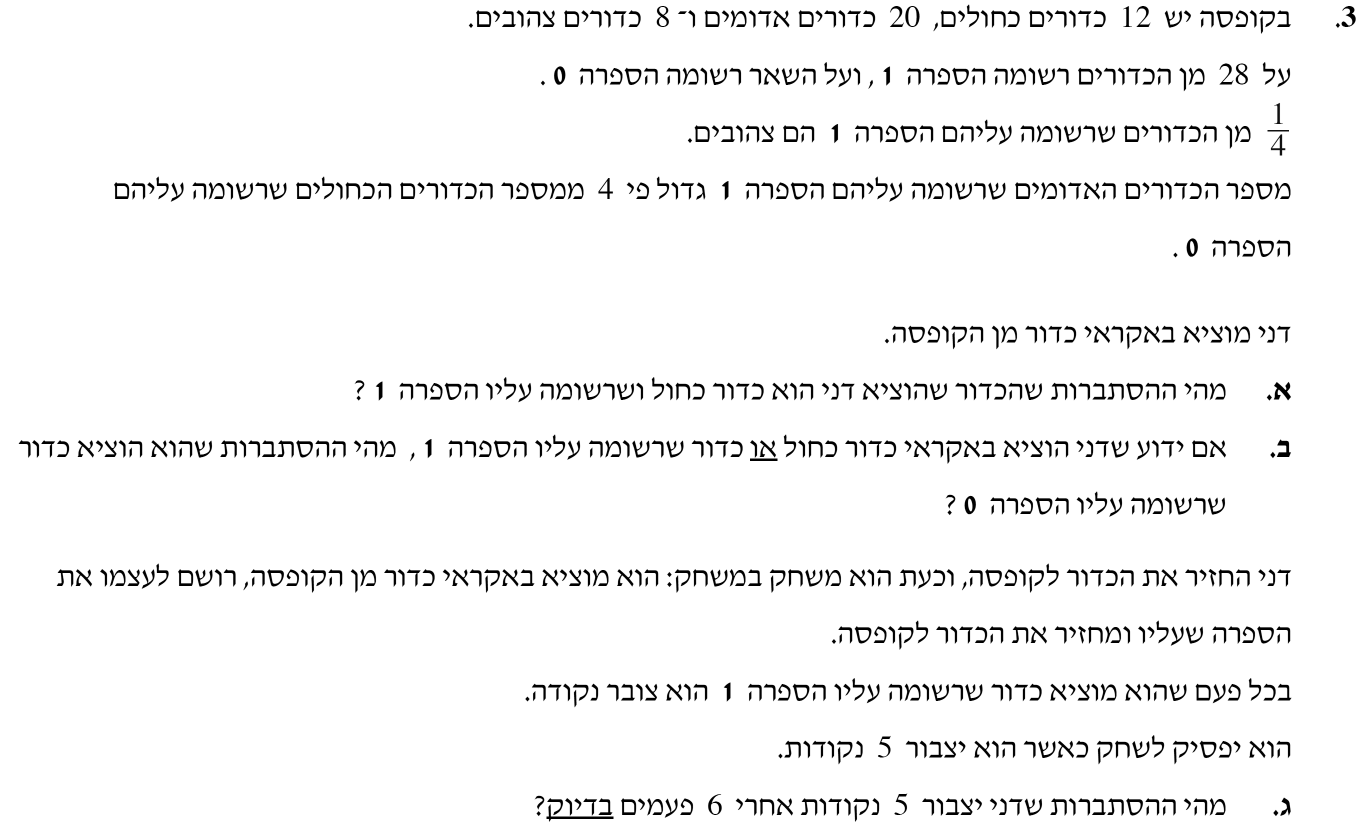
\includegraphics[width=.85\textwidth]{summer-2019b-3}
\end{center}

נסמן את המאורעות:
$K$
כדורים כפולים, 
$A$
כדורים אדומים,
$Z$
כדורים צהובים,
$0$
הספרה אפס,
$1$
הספרה אחד. השאלה שואלת על מאורעות המורכבים משני סוגי מאורעותת פשוטים יותר, צבעים וספרות, ולכן נארגן את המידע בטבלה.%
\footnote{%
באתר של יואל גבע הפתרון מתבסס על עץ. לדעתי שיטה זו מתאימה יותר כאשר יש מאורעות עוקבים, כגון שליפת הצבע מקופסה אחת ואחר כך שליפת הספרה מקופסה שנייה. כאן כאשר הניסוי הוא שליפה של כדור אחד עדיף להשתמש בטבלה.} בטבלה נרשום מספרים שלמים כאשר הכוונה של המספר 
$n$
הוא 
$P(n/40)$.

מספר הכדורים מכל צבע נתון ונתון גם שרבע מהכדורים שרשומה עליהם 
$1$
הם צהובים. ממידע זה ניתן למלא את התאים בטבלה בהם מופיעים מספרים שלמים. נסמן בנעלם
$X$
את מספרם של הכדורים הכחולים שרשומה עליהם אפס. לפי היחס הנתון בין 
$X$
לבין מספר הכדורים האדומים שרשומה עליהם אחד ניתן להשלים את הטבלה. מהתאים עבור הכדורים האדומים נקבל משוואה
$4X+11-X=20$
ולכן 
$X=3$.

\begin{center}
\selectlanguage{english}
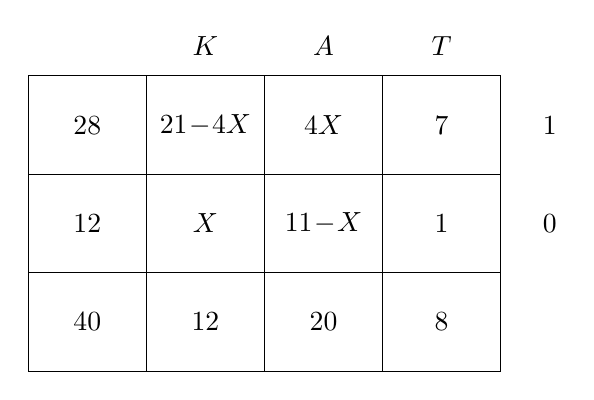
\begin{tikzpicture}[scale=1.25]
\draw (0,0) grid[xstep=1.2cm] (4.8,3);
\node at (4.2,3.3) {$\bm{T}$};
\node at (3,3.3) {$\bm{A}$};
\node at (1.8,3.3) {$\bm{K}$};
\node at (5.3,2.5) {$\bm{1}$};
\node at (5.3,1.5) {$\bm{0}$};

\node at (4.2,2.5) {$7$};
\node at (3,2.5) {$4X$};
\node at (1.8,2.5) {$21\!-\!4X$};
\node at (0.6,2.5) {$28$};

\node at (4.2,1.5) {$1$};
\node at (3,1.5) {$11\!-\!X$};
\node at (1.8,1.5) {$X$};
\node at (0.6,1.5) {$12$};

\node at (4.2,0.5) {$8$};
\node at (3,0.5) {$20$};
\node at (1.8,0.5) {$12$};
\node at (0.6,0.5) {$40$};

\end{tikzpicture}
\end{center}

\newpage

נציב 
$X=3$
ונקבל מספרים בכל התאים:
\begin{center}
\selectlanguage{english}
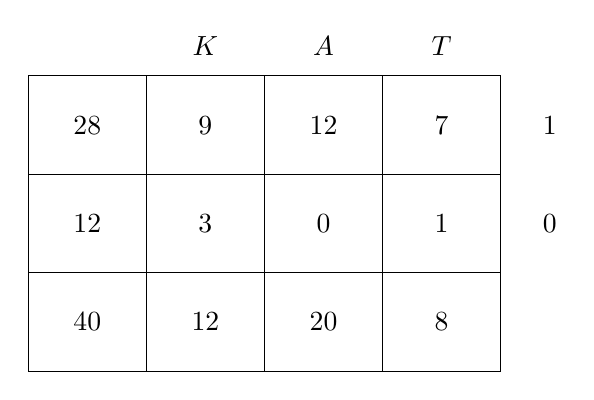
\begin{tikzpicture}[scale=1.25]
\draw (0,0) grid[xstep=1.2cm] (4.8,3);
\node at (4.2,3.3) {$\bm{T}$};
\node at (3,3.3) {$\bm{A}$};
\node at (1.8,3.3) {$\bm{K}$};
\node at (5.3,2.5) {$\bm{1}$};
\node at (5.3,1.5) {$\bm{0}$};

\node at (4.2,2.5) {$7$};
\node at (3,2.5) {$12$};
\node at (1.8,2.5) {$9$};
\node at (0.6,2.5) {$28$};

\node at (4.2,1.5) {$1$};
\node at (3,1.5) {$0$};
\node at (1.8,1.5) {$3$};
\node at (0.6,1.5) {$12$};

\node at (4.2,0.5) {$8$};
\node at (3,0.5) {$20$};
\node at (1.8,0.5) {$12$};
\node at (0.6,0.5) {$40$};

\end{tikzpicture}
\end{center}
\textbf{סעיף א}

מהטבלה נקבל
$P(K \cap 1) = \frac{9}{40}$.

\textbf{סעיף ב}

"אם ידוע" מכוון להתסברות מותנית:
\[
P(0/ K\:\cup\: 1) = \frac{P(0 \cap (K\:\cup\:1))}{P(K\:\cup\:1))}\,.
\]
אפשר לפתח את הביטוי לפי חוק הפילוג לקבוצות אבל פשוט נשים לב שלא יכול להיות כדור שרשומה עליו גם אפס וגם אחד, ולכן:
\[
P(0/ K\:\cup\: 1) = \frac{P(0 \cap K)}{P(K\:\cup\:1))}
= \frac{3}{12+28-9}=\frac{3}{31}\,.
\]
כאשר מחשבים את איחוד הקבוצות
$K, 1$
על ידי סכום מספר האיברים בקבוצה 
$K$
ומספר האיברים בקבוצה
$1$,
אנו סופרים את האיברים ב-%
$K\cap1$
פעמיים ולכן יש להחסיר את מספר האיברים בקבוצה זו.

\textbf{סעיף ג}

המילה "בדיוק" מכוון לנוסחת ברנולי אבל יש כאן מלכודת. לו שאלו מה ההסתברות לצבור חמש נקודות בחמשה סיבובים הפתרון מתקבל מנוסחת ברנולי פשוט. אבל כדי לקבל חמש נקודות בששה סיבובים חייבים להפסיד בסיבוב אחד בדיוק מבין חמשת הסיבובים הראשונים ורק אז לזכות בנקודה בסיבוב האחרון. אחרת, המשחק היה נפסק לאחר הסיבוב החמישי. נסמן ב-%
$k/n$
את המאורע של לזכות ב-%
$k$
נקודות מתוך 
$n$
סיבובים:
\[
P(\textrm{\R{זכייה חמישית בסיבוב הששי}})=P(4/5) P(1/1)=
{5 \choose 1}\left(\frac{12}{40}\right)^1\left(\frac{28}{40}\right)^4\left(\frac{28}{40}\right)^1=0.252015\,.
\]

%%%%%%%%%%%%%%%%%%%%%%%%%%%%%%%%%%%%%%%%%%%%%%%%%%%%%%%%%%%%%

\section{קיץ תשע"ט מועד א}

\begin{center}
\selectlanguage{english}
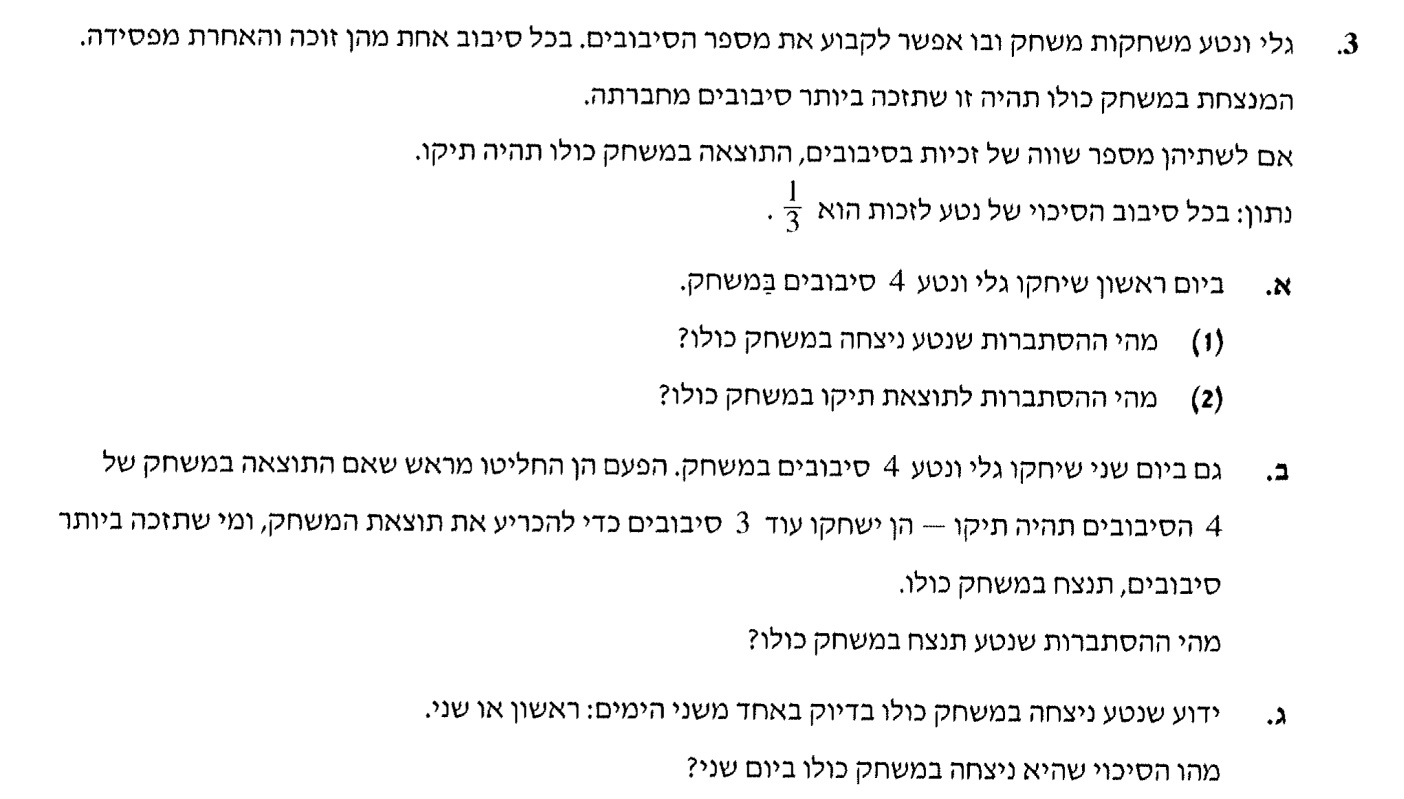
\includegraphics[width=.9\textwidth]{summer-2019a-3}
\end{center}

משחק בסיבובים מכוון לנוסחת ברנולי.

\textbf{סעיף א 1}

נסמן את המאורע שנטע ניצחה בסיבוב ב-%
$N$
והמאורע שנטע ניצחה במחשק ב-%
$M$.
\[
P(M) = P(N=3 \:\cup\: N=4)=P(N=3)+P(N=4)\,,
\]
כי במאורעות בלתי-תלויים: אי-אפשר לנצח גם בשלושה סיבובים וגם בארבעה. לפי נוסחת ברנולי:
\[
P(M)={4\choose 3}\left(\frac{1}{3}\right)^3\left(\frac{2}{3}\right)^1+
{4\choose 4}\left(\frac{1}{3}\right)^4\left(\frac{2}{3}\right)^0=
\frac{8}{81}+\frac{1}{81}=\frac{9}{81}=\frac{1}{9}\,.
\]

\textbf{סעיף א 2}

כדי להגיע לתיקו נטע חייבת לנצח בדיוק בשני סיבובים:
\[
P(N=2)={4\choose 2}\left(\frac{1}{3}\right)^2\left(\frac{2}{3}\right)^2=\frac{24}{81}=\frac{8}{27}\,.
\]

\textbf{סעיף ב}

נטע מנצחת במשחק אם היא מנצחת בארבעה סיבובים או שיש תיקו ואחכ כך היא מנצחת בשניים מתוך שלושה סיבובים. נשתמש בתוצאות של סעיף א ונקבל:
\begin{eqnarray*}
P(M)&=&\frac{1}{9}+\frac{8}{27}
  \left[{3\choose 2}\left(\frac{1}{3}\right)^2\left(\frac{2}{3}\right)^1  +
  {3\choose 3}\left(\frac{1}{3}\right)^3\left(\frac{2}{3}\right)^0
  \right]\\
  &=&\frac{1}{9}+\frac{8}{27}
  \left[ \frac{6}{27} + \frac{1}{27} \right]=
  \frac{81}{729}+\frac{56}{729}=\frac{137}{729}\,.
\end{eqnarray*}

\textbf{סעיף ג}

חייבים לשים לב לניסוח בסעיף ב': המשחק עם שבעה סיבובים מתרחש רק ביום שני כאשר ביום ראשון המחשק נשאר עם ארבעה סיבובים. נסכם את מה שיש לנו כאשר 
$N1, N2$
מסמנים שנטע ניצחה ביום ראשון ויום שני בהתאמה:
\[
P(N1) = \frac{1}{9},\quad P(\overline{N1})=\frac{8}{9},\quad 
P(N2) = \frac{137}{729}, \quad P(\overline{N2})=\frac{592}{729}\,.
\]
נניח ששני המשחקים בלתי-תלויים כך שאפשר להכפיל את ההסתברויות שלהם. 
נסמן ב-%
$1$
את המאורע שנטע מנצחת רק באחד משני המשחקים ונשמתש בעובדה ש-%
$(\overline{N1}\cup N2) \subseteq 1$,
כי ניצחון של נטע רק במשחק בשני הוא אחד המקרים של נטע מנצחת רק במשחק אחד. נחשב את ההסתברות המבוקשת:
\begin{eqnarray*}
P(\overline{N1}\cup N2) / 1) &=& 
\frac{P((\overline{N1}\cup N2) \cap 1)}{P(1)}\\
&=& \frac{P(\overline{N1})P(N2)}
{P(\overline{N1})P(N2)+P(N1)P(\overline{N2})}\\[8pt]
&=&\frac{\disfrac{8}{9}\cdot \frac{137}{729}}
{\disfrac{8}{9}\cdot \frac{137}{729}+\disfrac{1}{9}\cdot \frac{592}{729}}\\[8pt]
&=&\frac{8\cdot 137}{8\cdot 137+592}=\frac{1096}{1688}=0.6493\,.
\end{eqnarray*}

%%%%%%%%%%%%%%%%%%%%%%%%%%%%%%%%%%%%%%%%%%%%%%%%%%%%%%%%%

\newpage

\section{חורף תשע"ט}

\begin{center}
\selectlanguage{english}
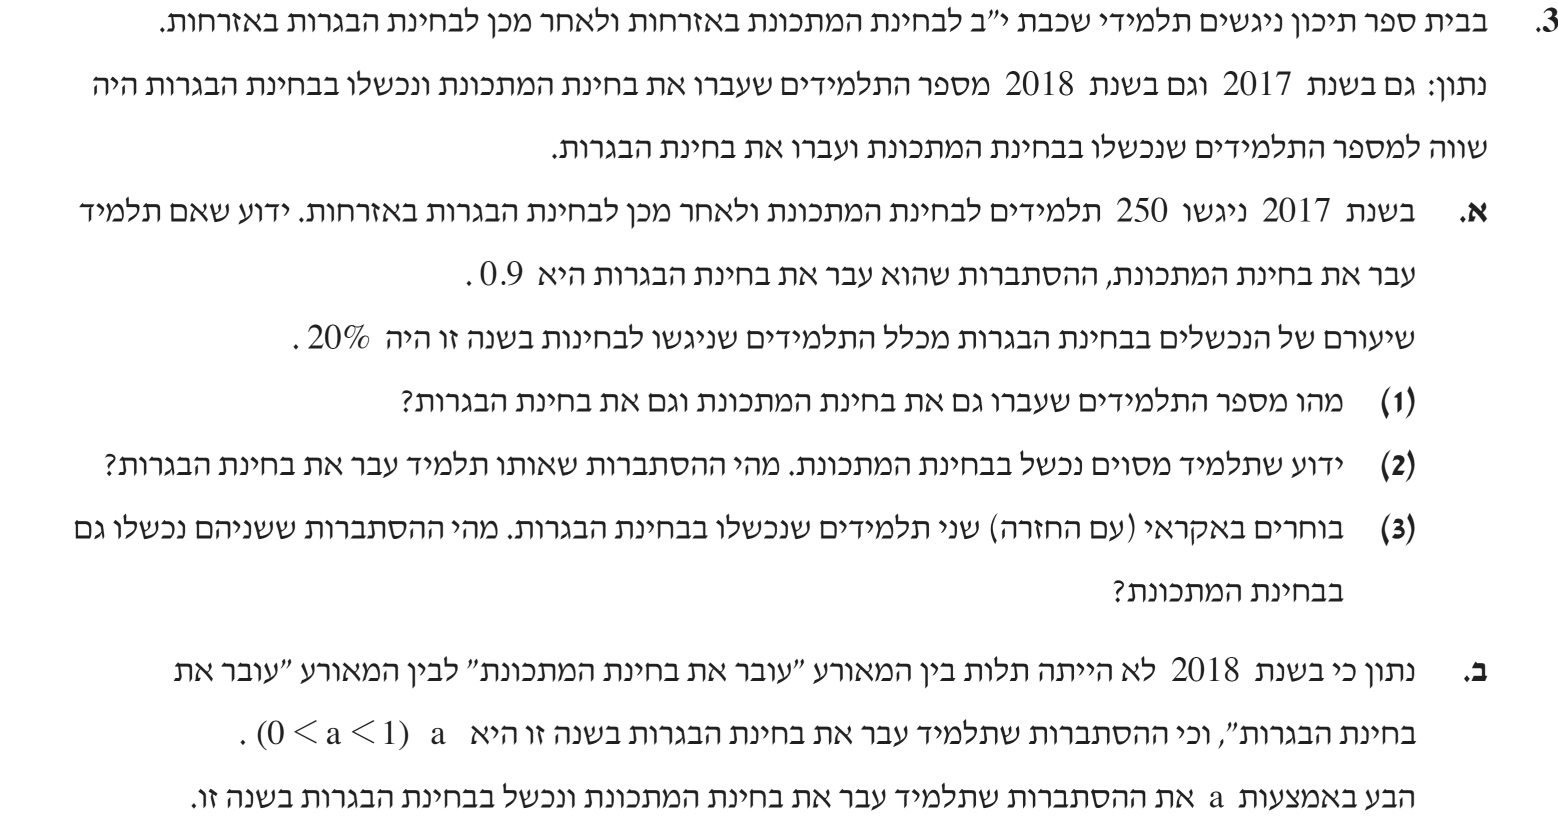
\includegraphics[width=.85\textwidth]{winter-2019-3}
\end{center}

השאלה שואלת על שני סוגי של מאורעות שמכוון לאירגון המידע בטבלה. נסמן ב-%
$B$ \L{bagrut}
את המאורע של הצלחה בבגרות ונסמן ב-%
$M$ \L{matkonet}
את המאורע של הצלחה במתכונת.

נתון שמספר הנכשלים בבגרות הוא 
$0.20$
ומהסתברות משלימה מספר העוברים הוא
$0.80$.
נתון גם ש:
\[
P(B\cap\overline{M})=P(\overline{B}\cap M)\,,
\]
ונסמן נעלם זה ב-%
$X$
ונסמן את הנעלם
$P(M)$
ב-%
$Y$.

המילה "ידוע" מכוון להסתברות מותנית:
\begin{eqnarray*}
P(B/M)&=&\frac{P(B\cap M)}{P(M)}=0.90\\
P(B\cap M)&=&0.90 P(M)=0.90Y\,.
\end{eqnarray*}
כעת ניתן למלא את כל תאי הטבלה:
\begin{center}
\selectlanguage{english}
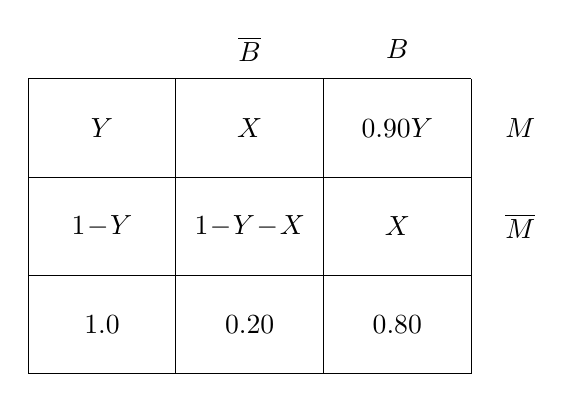
\begin{tikzpicture}[scale=1.25]
\draw (0,0) grid[xstep=1.5] (4.5,3);
\node at (3.75,3.3) {$B$};
\node at (2.25,3.3) {$\overline{B}$};
\node at (5,2.5) {$M$};
\node at (5,1.5) {$\overline{M}$};

\node at (3.75,2.5) {$0.90Y$};
\node at (2.25,2.5) {$X$};
\node at (0.75,2.5) {$Y$};

\node at (3.75,1.5) {$X$};
\node at (2.25,1.5) {$1\!-\!Y\!-\!X$};
\node at (0.75,1.5) {$1\!-\!Y$};

\node at (0.75,0.5) {$1.0$};
\node at (2.25,0.5) {$0.20$};
\node at (3.75,0.5) {$0.80$};
\end{tikzpicture}
\end{center}

מהעומדות של הבגרות נקבל שתי משוואות:
\begin{eqnarray*}
0.90Y+X&=&0.80\\
X+1-Y-X&=&0.20\\
Y&=&0.80\\
X&=&0.08\,.
\end{eqnarray*}
ניתן למלא אל כל התאים במספרים:
\begin{center}
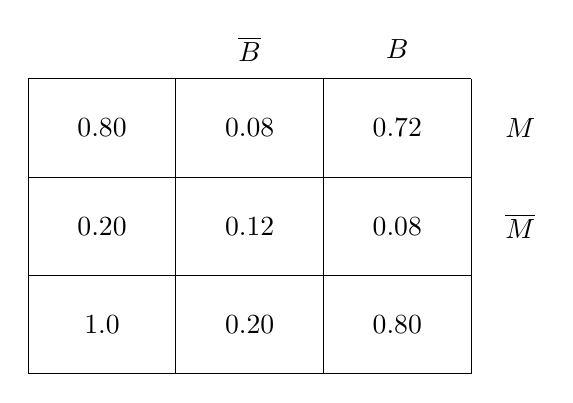
\begin{tikzpicture}[scale=1.25]
\draw (0,0) grid[xstep=1.5] (4.5,3);
\node at (3.75,3.3) {$B$};
\node at (2.25,3.3) {$\overline{B}$};
\node at (5,2.5) {$M$};
\node at (5,1.5) {$\overline{M}$};

\node at (3.75,2.5) {$0.72$};
\node at (2.25,2.5) {$0.08$};
\node at (0.75,2.5) {$0.80$};

\node at (3.75,1.5) {$0.08$};
\node at (2.25,1.5) {$0.12$};
\node at (0.75,1.5) {$0.20$};

\node at (0.75,0.5) {$1.0$};
\node at (2.25,0.5) {$0.20$};
\node at (3.75,0.5) {$0.80$};
\end{tikzpicture}
\end{center}

\textbf{סעיף א 1}

מהטבלה
$P(B\cap M)=0.72$
ומספר הנבחנים
$250=$
ולכן מספר העוברים את שתי הבחינות
$180=$.

\textbf{סעיף א 2}

\[
P(B/\overline{M})=\frac{P(B\cap\overline{M})}{P(\overline{M})}=
\frac{0.08}{0.2}=0.4\,.
\]

\textbf{סעיף א 3}

\[
P(\overline{M}/\overline{B})=\frac{P(\overline{M}\cap \overline{B})}{P(\overline{B})}=\frac{0.12}{0.2}=0.6\,.
\]

\textbf{סעיף ב}

בתחילת השאלה כתוב ש-%
$P(M\cap\overline{B})=P(\overline{M}\cap B)$
גם עבור שנת 2018. המאורעות
$M,B$
בלתי-תלויים ולכן גם המאורעות
$M,\overline{B}$
ו-%
$\overline{M},B$.
נמצא בחישוב את הביטוי המבוקש ל-%
$P(M\cap\overline{B})$:
\begin{eqnarray*}
P(M) P(\overline{B})&=&P(M\cap\overline{B})=
P(\overline{M}\cap B)=P(\overline{M})P(B)\\
P(M)(1-a)&=&(1-P(M))a\\
P(M)&=&a\\
P(M\cap\overline{B})&=&P(M)P(\overline{B})=a(1-a)=a-a^2\,.
\end{eqnarray*}
